\chapter{Экспериментальный раздел}
В данном разделе проводится анализ врмени выполнения запросов в зависимости от наличия индексов. Все исследования проводились на таблицах, состоящих из 1000 записей. Для повышения производительности используются B-tree индексы, так как с помощью B-дерева можно проиндексировать любые данные, которые могут быть отсортированы, т. е. для которых применимы операции сравнения больше/меньше/равно.

\section{Поиск по первичному ключу}
Выполним следующий запрос:
\begin{lstlisting}[label=lst:pk_1, caption=Запрос поиска по первичному ключу, language=sql]
select * from Account where id = 1;
\end{lstlisting}

\begin{figure}[h!]
	\begin{center}
		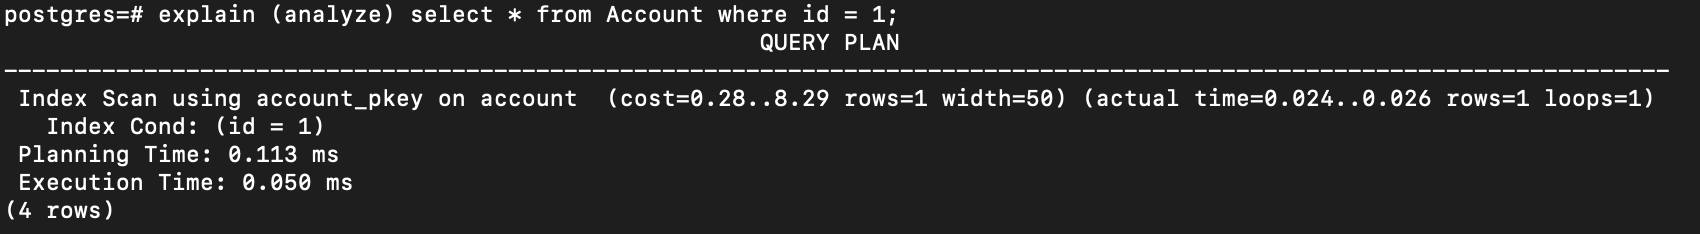
\includegraphics[width = \linewidth]{img/pk.png}
	\end{center}
	\captionsetup{justification=centering}
	\caption{Поиск по первчиному ключу без индекса}
	\label{img:get-example}
\end{figure}

Создадим индекс:

\begin{lstlisting}[label=lst:pk_1, caption=Создание индекса для поиска по первичному ключу, language=sql]
create index id_idx on account using btree(id);
\end{lstlisting}

\begin{figure}[h!]
	\begin{center}
		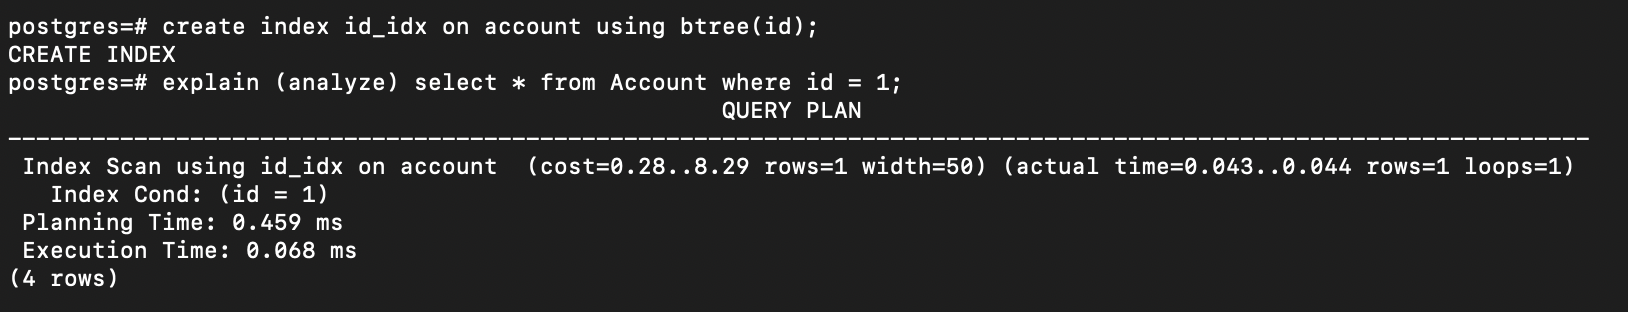
\includegraphics[width = \linewidth]{img/pk_idx.png}
	\end{center}
	\captionsetup{justification=centering}
	\caption{Поиск по первчиному ключу с индексом}
	\label{img:get-example}
\end{figure}

Видим, что время выполнения запроса почти не изменилось, что говорит о том, что для первичного ключа индекс создаётся автоматически, поэтому создание ещё одного индекса не приведёт к повышению производительности.

\section{Поиск по таблице с фильтрацией}
Выполним следующий запрос:
\begin{lstlisting}[label=lst:field_1, caption=Запрос поиска с фильтрацией, language=sql]
select id, login, password, name, role from account where name = 'Eric';
\end{lstlisting}

\begin{figure}[h!]
	\begin{center}
		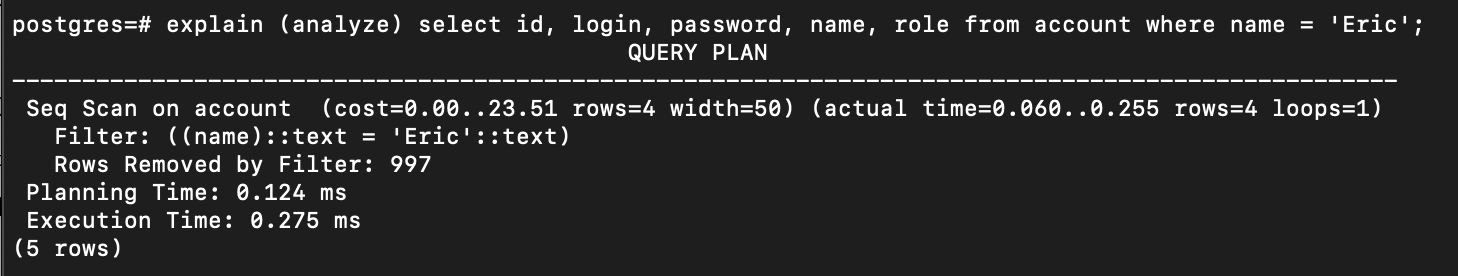
\includegraphics[width = \linewidth]{img/field.png}
	\end{center}
	\captionsetup{justification=centering}
	\caption{Поиск с фильтрацией без индекса}
	\label{img:get-example}
\end{figure}

Создадим индекс:

\begin{lstlisting}[label=lst:pk_1, caption=Создание индекса для поиска с фильтрацией, language=sql]
create index name_idx on account using btree(name);
\end{lstlisting}

\begin{figure}[h!]
	\begin{center}
		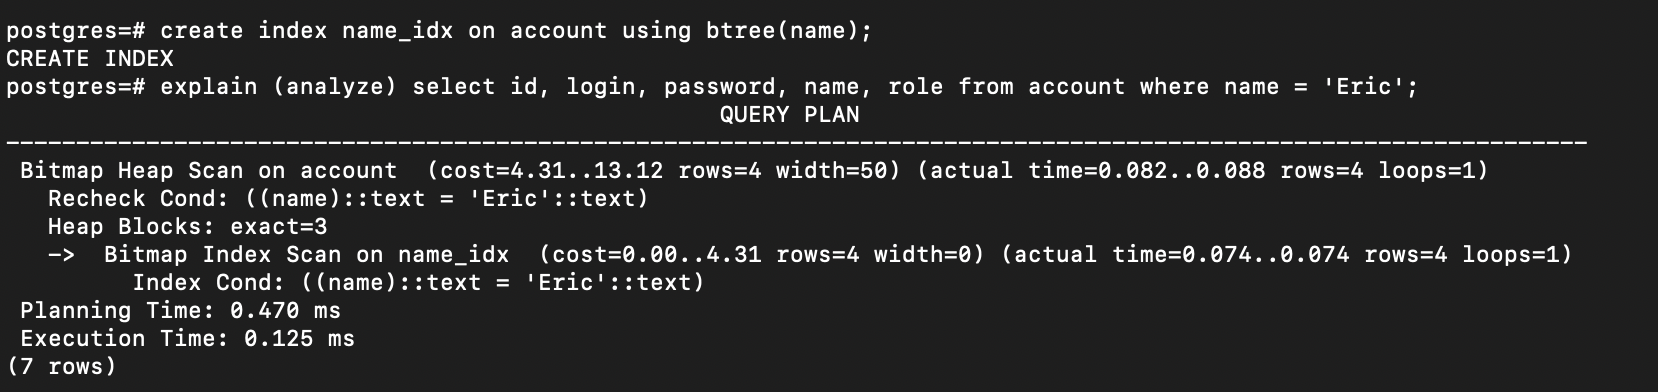
\includegraphics[width = \linewidth]{img/field_idx.png}
	\end{center}
	\captionsetup{justification=centering}
	\caption{Поиск с фильтрацией с индексом}
	\label{img:get-example}
\end{figure}

Видим, что время выполнения запроса уменьшилось в 2.2 раза, что говорит о том, что создание индекса приводит к повышению производительности. 

\newpage
\section{Поиск по внешнему ключу при объединении таблиц}
Выполним следующий запрос:
\begin{lstlisting}[label=lst:fk, caption=Запрос поиска по внешнему ключу при объединении таблиц, language=sql]
select bookitem.id, name, author from bookitem join book on book.id = bookitem.book_id where bookitem.book_id = 5;
\end{lstlisting}

\begin{figure}[h!]
	\begin{center}
		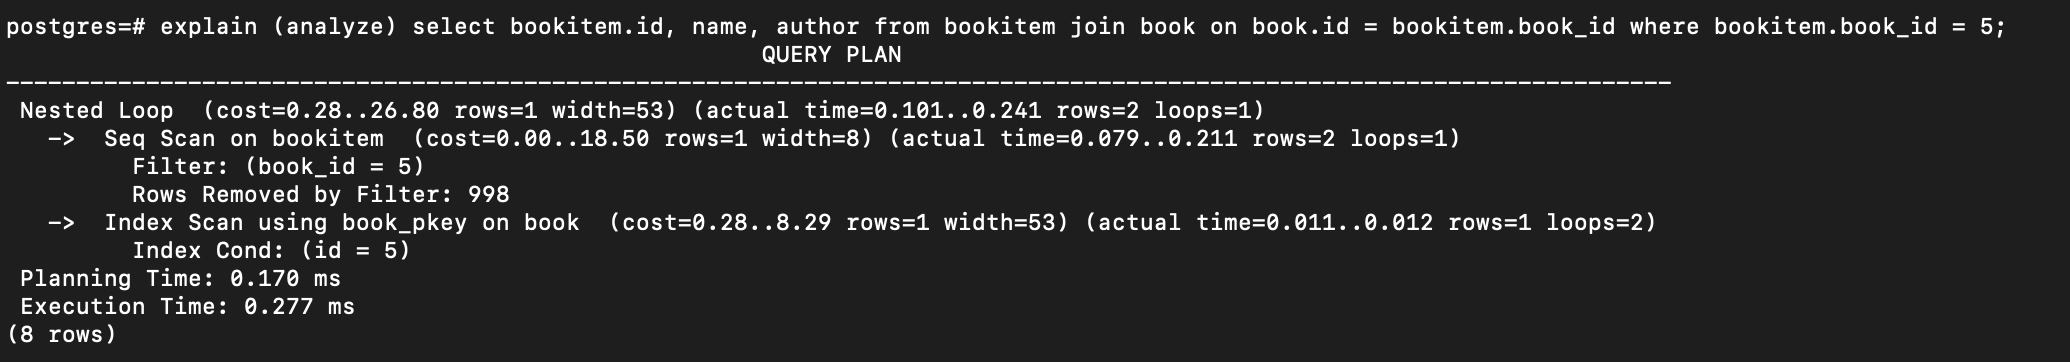
\includegraphics[width = \linewidth]{img/fk.png}
	\end{center}
	\captionsetup{justification=centering}
	\caption{Поиск по внешнему ключу при объединении таблиц без индекса}
	\label{img:get-example}
\end{figure}

Создадим индекс:

\begin{lstlisting}[label=lst:fk_idx, caption=Создание индекса для поиска по внешнему ключу при объединении таблиц, language=sql]
create index ind_book_id on bookitem using btree(book_id);
\end{lstlisting}

\begin{figure}[h!]
	\begin{center}
		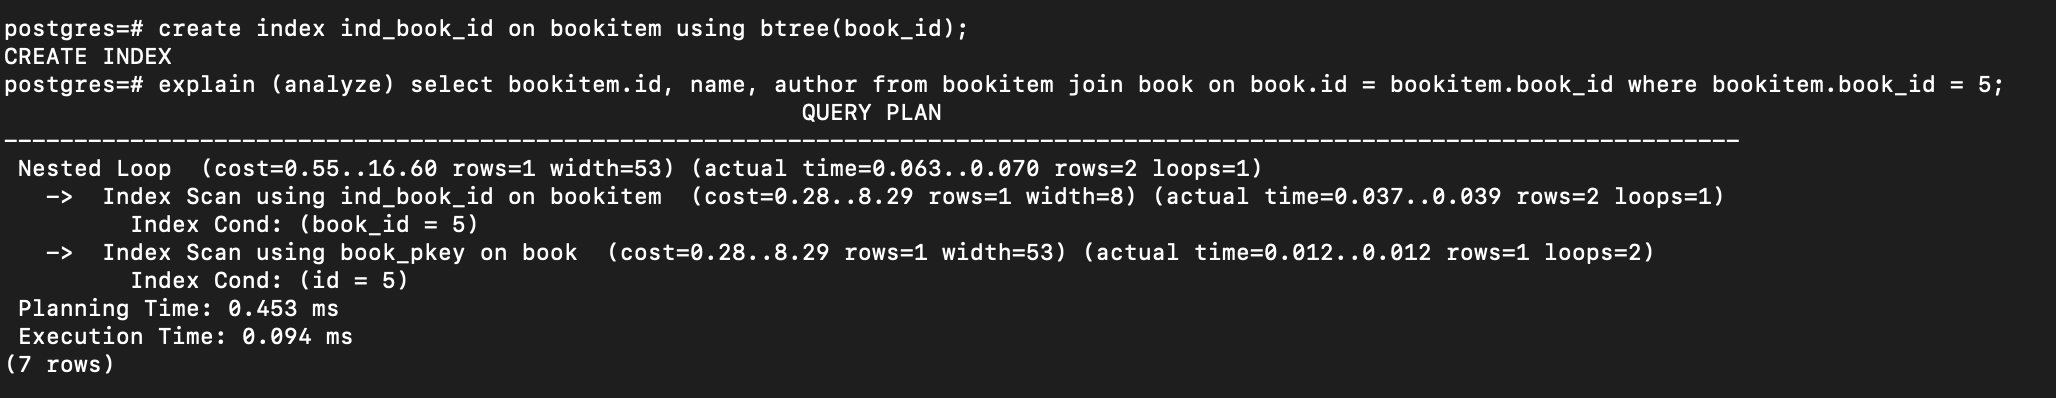
\includegraphics[width = \linewidth]{img/fk_idx.png}
	\end{center}
	\captionsetup{justification=centering}
	\caption{Поиск по внешнему ключу при объединении таблиц с индексом}
	\label{img:get-example}
\end{figure}

Видим, что время выполнения запроса уменьшилось в 2.95 раза, что говорит о том, что создание индекса приводит к повышению производительности. 

\section*{Вывод}
\addcontentsline{toc}{section}{Вывод}
В результате исследования было выяснено, что использование индексов в большинстве случаев повышает производительность выполнения запросов. 